\documentclass[11pt]{article}
\usepackage{mathptmx}
\usepackage{geometry}
\usepackage{paralist}
\usepackage{amsmath}
\usepackage{amsfonts}
\usepackage{ascmac}
\usepackage{bm}
\usepackage[]{subcaption}
\usepackage[dvipdfmx]{graphicx, color}
\usepackage{verbatim}
\usepackage{natbib}
\usepackage{color}
\usepackage{setspace}

\DeclareMathOperator*{\argmin}{arg\,min}
\DeclareMathOperator*{\argmax}{arg\,max}

\begin{document}
\setstretch{1.0}

\title{Comparison of Option Hedging Strategies Using Deep Q Network and Deep Deterministic Policy Gradient with the Time-Discretized Black-Scholes-Merton Model with Transaction Costs}

\author{Yuki Yasuda}

\date{\today}

\maketitle

\begin{abstract}
   This report investigates option hedging strategies with the Black-Scholes-Merton model with transaction costs, using two reinforcement learning algorithms: Deep Q Network (DQN) and Deep Deterministic Policy Gradient (DDPG). The DQN is simple and applied to a problem with a discrete action space, while the DDPG is complicated and applied to a problem with a continuous action space. An agent hedges 100 call options with fixed strike and expiry, where the underlying stock price obeys the geometric Brownian motion. The case of no transaction costs is first discussed to examine the convergence of policy. In this case, the optimal policy is the delta hedging. The DDPG policy is closer to the delta hedging than the DQN. The case of non-zero transaction costs is next examined. The DDPG and the DQN agent tend to reduce the number of shares of stock in their positions to cut the transaction costs when the option is in the money (ITM). The DDPG agent has a smaller number of shares of stock, in the case of not only ITM but also OTM (out of the money). The DQN agent changes a number of shares of stock not frequently. The results reveal that the hedging strategy of the DQN is statistically different from that of the DDPG.   
\end{abstract}


\section{Introduction}

European call options have been traded over the world since the Black-Scholes-Merton (BSM) model was derived \citep{Shreve:2008}. Pricing or hedging an option is categorized into stochastic optimal control problems. In these days, reinforcement learning (RL) \citep{Sutton:Barto:2018} has been rapidly developed, influenced by the development of deep learning \citep{Goodfellow:etal:2018}. RL is a method to solve stochastic optimal control problems. It may be natural to apply RL algorithms to hedge or price options.

Halperin \citep{Halperin:2017, Halperin:2018} discussed how to develop the time-discretized BSM model with a RL techniques named Q-learning \citep{Watkins:Dayan:1992}. He showed that both the option pricing and hedging can be performed within a framework of the action-value function ($Q$ function). We tried to develop his theory to the time-discretized BSM model with transaction costs, however, the theory became too complicated (not shown in detail).  The main reason for the complication is that both hedging and pricing options are performed within one framework of the Q-learning.

Kolm and Ritter \citep{Kolm:Ritter:2019} developed a different theory of option hedging with the Q-learning. They separated hedging from pricing and discussed how to hedge an option that is priced with the (continuous-time) BSM model in a realistic market where time is discrete and transaction costs are not zero. Their theory is easily applied to not only European options but also more complicated derivatives. However, in their theory, the number of shares of stock in the hedger position must be treated as an integer, even if its value is quite large [e.g., $O(10^5)$], because the Q-learning cannot be applied to a problem with a continuous action space. It would be more practical to regard the number of shares of stock as continuous, particularly in a larger brokerage securities.

In this report, we applied both the Q-learning and the Deep deterministic policy gradient (DDPG) algorithm to the option hedging and compare both hedging strategies. DDPG is a RL algorithm that can solve a problem with a continuous action space \citep{Silver:etal:2014, Lillicrap:etal:2015}. This report is organized as follows. In Section 2, the Q-learning (deep Q network) and the DDPG are briefly reviewed. An idealized market and a problem of hedging options are constructed in Section 3 on the basis of the theories of Halperin \citep{Halperin:2017, Halperin:2018} and Kolm and Ritter \citep{Kolm:Ritter:2019}. Numerical experiments are performed in Section 4, and we compare the hedging strategies. In Section 5, we finally summarize the results obtained in this report.


\section{Brief summary on reinforcement learning}

We briefly summarize the framework of reinforcement learning (RL) with Markov decision process \citep{Sutton:Barto:2018} and then review the two RL algorithms used in this report: Deep Q Network (DQN) \citep{Watkins:Dayan:1992, Mnih:etal:2013} and Deep Deterministic Policy Gradient (DDPG) \citep{Silver:etal:2014, Lillicrap:etal:2015}.

\subsection{Markov decision process and Bellman equations}

RL is a method to solve multi-period optimal control problems. An optimal control problem can be formulated using agent and environment. The agent determines an action $a_t$ at every time $t$, following its policy $\pi$ and the current state $s_t$. The environment gives the next state $s_{t+1}$ and the reward $r_t$ based on the agent action $a_t$ and the current state $s_{t}$, where the transition probability is denoted by $p(s_{t+1} \mid s_t, a_t)$ and $r_t$ is a function of $s_t$, $a_t$, and $s_{t+1}$. The process is repeated from $t=0$ to $t=T$. The objective of RL is to obtain the optimal policy $\pi^\ast$ that maximizes the cumulative sum of discounted rewards:
%
\begin{equation}
	R_{0} = \sum_{t=0}^{T} {\gamma}^t r_t(s_t, a_t, s_{t+1}),
\end{equation}
%
where $\gamma$ is a discount rate ($0 < \gamma < 1$) and $r_T$ is determined only by $s_{T}$.

The action-value function is introduced to solve the control problem:
%
\begin{equation}
	q_{t}^{\pi}(s,a) := \mathbb{E}[R_t \mid s_t = s, a_t = a], \label{bellman_equation}
\end{equation}
%
where $R_t := \sum_{t'=t}^{T} {\gamma}^{t'-t} r_{t'}$. Using the tower rule, we obtain the Bellman equation:
%
\begin{equation}
	q_{t}^{\pi}(s,a) = \mathbb{E}\left[  r_{t} + \gamma q_{t+1}^{\pi}(s', a') \;\middle|\; s_t = s, a_t = a\right].
\end{equation}
%
The optimal policy $\pi^\ast$ gives the maximum action-value function $q^{\ast}_t(s,a)$ for any $t$, $s$, and $a$:
%
\begin{equation}
	q^{\ast}_t(s,a) \ge q_{t}^{\pi}(s,a).
\end{equation}
%
The function of $q^{\ast}_t(s,a)$ satisfies the Bellman optimality equation:
%
\begin{equation}
	q^{\ast}_t(s,a) = \mathbb{E}\left[  r_{t} + \gamma \max_{a'} q_{t+1}^{\ast}(s', a') \;\middle|\; s_t = s, a_t = a\right]. \label{bellman_optimality_equation}
\end{equation}

The optimal policy $\pi^\ast$ is obtained in principle by solving the Bellman optimality equation (\ref{bellman_optimality_equation}). According to the contraction mapping theorem, the unique solution exists for the Bellman optimality equation, which is $q^{\ast}_t(s,a)$. The optimal policy is then given by $\pi^\ast = \argmax_{a} q_t^{\ast}(s,a)$ for any $t$ and $s$. However, solving the Bellman optimality equation is quite difficult because the transition probability $p(s_{t+1} \mid s_{t}, a_{t})$ is often unknown and the dimension of state $s$ or action $a$ is quite large (sometimes continuous) in most cases. We have to apply some approximation and sampling methods to obtain the optimal policy.

\subsection{Deep Q network (DQN)}

Deep Q Network (DQN) \citep{Mnih:etal:2013} is a combination of deep learning \citep{Goodfellow:etal:2018} and Q-learning \citep{Watkins:Dayan:1992}. DQN is often applied to a problem in which state is continuous, action is discrete, and the transition probability is unknown. The optimal action-value function is approximated with a deep neural network: $q^\ast_t(s,a) \approx q^\ast_t(s,a; \bm{w})$, where $\bm{w}$ represents the weight parameters in the deep network. The Bellman optimality equation is solved by sampling data $(s_t, a_t, r_t, s_{t+1})$ from some buffer. The DQN algorithm is in the following \citep{Mnih:etal:2013}.

\vspace{1zw}

\begin{itembox}[l]{Algorithm of Deep Q Network (DQN) \citep{Mnih:etal:2013}}
	Initialize replay buffer $RB$ \\
	Initialize action-value function $q^\ast$ with random weights $\bm{w}$ \\
	\textbf{for} episode $=$ $1$, $M$ \textbf{do} \\
	\hspace{2zw} Initialize sequence $s_0 = x_0$ \\
	\hspace{2zw} \textbf{for} $t = 0, T$ \textbf{do} \\
		\hspace{4zw} With probability $\epsilon$ select a random action $a_t$ \\
		\hspace{4zw} otherwise select $a_t = \argmax_{a'} q^{\ast}(s_t, a')$ \\
		\hspace{4zw} Execute action $a_t$ in the environment and observe $r_t$ and $s_{t+1}$ \\
		\hspace{4zw} Store transition $(s_t, a_t, r_t, s_{t+1})$ in $RB$ \\
		\hspace{4zw} Sample random mini-batch of transitions $(s_j, a_j, r_j, s_{j+1})$ from $RB$ \\
		\begin{equation}
		\text{Set } y_j = \begin{cases}
				r_j & \text{for terminal $s_{t+1}$} \\
				r_j + \gamma \max_{a'} q^{\ast} (s_{t+1}, a') & \text{for non-terminal $s_{t+1}$}
			\end{cases}
		\end{equation} \\
		\hspace{4zw} Perform a semi-gradient descent step on $(y_j - q^\ast(s_j, a_j; \bm{w}))^2$ \\
	\hspace{2zw} \textbf{end for} \\
	\textbf{end for}
\end{itembox}

\vspace{1zw}

\subsection{Deep deterministic policy gradient (DDPG)}

DQN is difficult to apply a problem in which both state and action are continuous because the optimal policy is given by $\pi^\ast = \argmax_{a'} q^\ast(s, a')$. Deep deterministic policy gradient (DDPG) algorithm can be applied to such a problem \citep{Silver:etal:2014, Lillicrap:etal:2015}. In DDPG, the optimal policy is a function of state $\mu(s, \bm{\theta}^\mu)$, which is represented by a deep network with weights $\bm{\theta}^\mu$. This function is obtained by optimizing the action-value function $q(s, a; \bm{\theta}^q)\mid_{a = \mu(s)}$, which is described by another deep network with weights $\bm{\theta}^q$. The function $\mu(s, \bm{\theta}^\mu)$ is updated according to the deterministic policy gradient theorem \citep{Silver:etal:2014}. The DDPG algorithm is in the following \citep{Lillicrap:etal:2015}.

\vspace{1zw}

\begin{itembox}[l]{Algorithm of Deep Deterministic Policy Gradient (DDPG) \citep{Lillicrap:etal:2015}}
	Randomly initialize critic network $q(s, a; \bm{\theta}^q)$ and actor $\mu(s; \bm{\theta}^\mu)$\\
	Initialize target network $q'$ and $\mu'$ with weights $\bm{\theta}^{q'} \leftarrow \bm{\theta}^{q}$ and $\bm{\theta}^{\mu'} \leftarrow \bm{\theta}^{\mu}$\\
	Initialize replay buffer $RB$\\
	\textbf{for} episode $=$ $1$, $M$ \textbf{do}\\
	\hspace{2zw} Initialize a random process $\xi_t$ (e.g., Ornstein-Uhlenbeck process) for action exploration\\
	\hspace{2zw} Receive initial observation state $s_0$\\
	\hspace{2zw} \textbf{for} $t = 0, T$ \textbf{do}\\
		\hspace{4zw} Select action $a_t = \mu(s_t; \bm{\theta}^\mu) + \xi_t$ according to the current policy \\
		\hspace{4zw} Execute action $a_t$ and observe reward $r_t$ and observe new state $s_{t+1}$ \\
		\hspace{4zw} Store transition $(s_t, a_t, r_t, s_{t+1})$ in $RB$ \\
		\hspace{4zw} Sample a random mini-batch of $n$ transitions $(s_j, a_j, r_j, s_{j+1})$ from $RB$ \\
		\hspace{4zw} Set $y_j = r_j + \gamma q'(s_{j+1}, \mu'(s_{j+1}; \bm{\theta}^{\mu'}); \bm{\theta}^{q'})$ \\
		\hspace{4zw} Update critic by minimizing the loss: $L = \frac{1}{n} \sum [y_j - q(s_j, a_j; \bm{\theta}^q)]^2$ \\
		\hspace{4zw} Update the actor policy using the sampled policy gradient:
		\begin{equation}
		\nabla_{\theta^{\mu}} J \approx \frac{1}{n}\sum \frac{\partial q(s_j,a; \bm{\theta}^q)}{\partial a} \mid_{a = \mu(s_j; \bm{\theta}^\mu)} \nabla_{\theta^{\mu}} \mu(s_j; \bm{\theta}^\mu)
		\end{equation}
		\hspace{4zw} Update the target networks:\\
		\begin{align}
			\bm{\theta}^{q'} &\leftarrow \tau \bm{\theta}^{q} + (1-\tau) \bm{\theta}^{q'} \\
			\bm{\theta}^{\mu'} &\leftarrow \tau \bm{\theta}^{\mu} + (1-\tau) \bm{\theta}^{\mu'}
		\end{align}
	\hspace{2zw} \textbf{end for}\\
	\textbf{end for}
\end{itembox}

\vspace{1zw}

\section{Time-discretized Black-Scholes-Merton model with transaction costs}

\subsection{Idealized market}

In this section, we formulate the time-discretized Black-Scholes-Merton (BSM) model with transaction costs. We consider the following idealized market:

\begin{itemize}
	\item Only the two assets exist: stock $S_t$ and riskless bank account $B_t$.
	\item The stock price $S_t$ obeys the geometric Brownian motion (\ref{SDE:Stock}).
	\item The shares of stock is represented by an integer.
	\item The risk-free interest rate $\rho$ is constant.
	\item The market has no holidays.
	\item The assets are traded at discrete time steps under the constraint of the self-financing condition.
	\item Transaction costs are described by a function $f := f(S_t, \delta N_t)$, where $\delta N_t$ is a change of the number of shares of stock $N_t$.
\end{itemize}

The geometric Brownian motion is
%
\begin{equation}
	\delta S_{t} = \mu S_t \; \delta t + \sigma S_t \; \delta W_t \label{SDE:Stock},
\end{equation}
%
where $\mu$ and $\sigma$ are constant and $W_t$ is a Wiener process. According to the self-financing condition, $B_{t+1}$ is given by
%
\begin{equation}
	B_{t+1} = B_t e^{\rho \delta t} - (N_{t+1} - N_{t}) S_t - f(S_t, \delta N_t), \label{Bt:self:financing}
\end{equation}
%
where $\delta N_t$ is equal to $N_{t+1} - N_{t}$. The time evolution and the portfolio rebalance are summarized in the following:
%
\begin{equation}
	\underbrace{(S_t, N_t, B_t e^{\rho \delta t})}_{\text{time } t} \quad \rightarrow \underbrace{(S_t, N_{t+1}, B_{t+1})}_{\text{time } t \text{ after rebalancing}} \rightarrow \quad \underbrace{(S_{t+1}, N_{t+1}, B_{t+1} e^{\rho \delta t})}_{\text{time } t+1}. \label{portfolio:evolution}
\end{equation}

The agent sells 100 European call options at $t=0$ with strike $K$ and expiry $T$ and hedges the 100 options until $t=T$ (i.e., the agent position is fixed). The option price is given by the (continuous-time) BSM model \citep{Shreve:2008}.

\subsection{State, action, and reward}

We re-formulate the above problem using the language of Markov decision process. The state $s_t$ is first introduced by combining the ideas of \citep{Halperin:2017, Halperin:2018} and \citep{Kolm:Ritter:2019}:
%
\begin{equation}
	s_t := \left(t, W_t, C_t, \Delta_t, N_t \right),
\end{equation}
%
where $t$ is the discretized time, $W_t$ is a Wiener process, $C_t$ is the option price given by the BSM model, $\Delta_t$ is the option delta multiplied by $100$ ($\Delta_t := 100 \times \frac{\partial C_t}{\partial S_t}$), and $N_t$ is the number of shares of stock in the portfolio. As the agent hedges the 100 call options, the delta neutral position is constructed by making $N_t$ equal to $\Delta_t$. The stock price $S_t$ is given by $W_t$:
%
\begin{equation}
	S_t = S_0 \exp \left[ \sigma W_t + \left(\mu - \frac{\sigma^2}{2} \right) t \right], \label{solution:SDE}
\end{equation}
%
which is the solution of the (continuous-time) geometric Brownian motion. The action $a_t$ is a number of shares of stock at $t+1$:
%
\begin{equation}
	a_t(s_t) := N_{t+1}. 
\end{equation}
%
Following (\ref{portfolio:evolution}), the Markov decision process is defined as
%
\begin{equation}
	\underbrace{\left(t, W_t, C_t, \Delta_t, N_t \right)}_{s_t \text{ at time } t} \quad \underset{a_t }{\longrightarrow} \quad \underbrace{\left(t, W_t, C_t, \Delta_t, N_{t+1} \right)}_{\text{time } t \text{ after taking action } a_t} \quad \underset{r_t }{\longrightarrow} \quad \underbrace{\left(t + 1, W_{t+1}, C_{t+1}, \Delta_{t+1}, N_{t+1} \right)}_{s_{t+1} \text{ at time } t+1},
\end{equation} 
%
where $r_t$ is a reward determined by $s_t$, $a_t$, and $s_{t+1}$. The state $s_t$ does not need to contain the bank account $B_t$ because (\ref{Bt:self:financing}) and (\ref{solution:SDE}) uniquely determine $B_t$ with the given state $s_t$.  

We finally specify the function of $r_t$ on the basis of \citep{Kolm:Ritter:2019}. The agent portfolio at time $t$ is described as
%
\begin{equation}
	\Pi_t = N_t S_t + B_t e^{\rho \delta t} - 100 \; C_t.
\end{equation}
%
The function $r_t$ is determined through the following cumulative sum of discounted rewards:
%
\begin{align}
	R_0 &:= \mathbb{E}\left[   (N_T S_T - N_0 S_0) + (100 C_0 - N_0 S_0) e^{\rho T}
	+ \sum_{t=0}^{T-1} \{B_{t+1} - B_t e^{\rho \delta t}\} e^{\rho (T-t)} - 100 C_T \right] \label{expected:return} \\
	&- \frac{\kappa}{2} {\rm Var} \left[ \Pi_T \right], \label{variance:sum:reward}
\end{align}
%
where the first term is the expected return and the second one is the variance of the portfolio (i.e., the magnitude of risk). The balance between return and risk is controlled by the constant of $\kappa$. The term of $(100 C_0 - N_0 S_0) e^{\rho T}$ represents that the agent makes a deposit at $t=0$ immediately after selling the 100 options. We set $N_0 = 0$ without loss of generality. The agent has to determine the initial portfolio immediately after selling the 100 options, i.e., the agent determines the initial number of shares of stock.

The return (\ref{expected:return}) is decomposed as follows:
%
\begin{align}
	&(N_T S_T - N_0 S_0) + \{ (100 C_0 - N_0 S_0) e^{\rho T} - 100 C_0 \} + \sum_{t=0}^{T-1} \{B_{t+1} - B_t e^{\rho \delta t}\} e^{\rho (T-t)} - 100 (C_T - C_0) \\
	&= \sum_{t=0}^{T-1} (N_{t+1} S_{t+1} - N_t S_t) + \{B_{t+1} - B_t e^{\rho \delta t}\} e^{\rho (T-t)} - 100 (C_{t+1} - C_t) \\
	&\quad+ \{ (100 C_0 - N_0 S_0) e^{\rho T} - 100 C_0 \} \\
	&= \sum_{t=0}^{T-1} (N_{t+1} S_{t+1} - N_t S_t) - \{ (N_{t+1}-N_t) S_t + f(S_t, \delta N_t) \} e^{\rho (T-t)} - 100 (C_{t+1} - C_t) \label{decomposition:return1} \\
	&\quad+ \{ (100 C_0 - N_0 S_0) e^{\rho T} - 100 C_0 \}, \label{decomposition:return2}
\end{align}
%
where the self-financing condition (\ref{Bt:self:financing}) is used.

The variance (\ref{variance:sum:reward}) is decomposed as follows:
%
\begin{align}
	{\rm Var} \left[ \Pi_T \right] &= {\rm Var} \left[ \sum_{t=0}^{T-1} \delta \Pi_t \right] \\
	&= \sum_{t=0}^{T-1}  {\rm Var} \left[ \delta \Pi_t \right] \\
	&= \sum_{t=0}^{T-1}  {\rm Var} \left[ N_{t+1} \delta S_t - 100 \delta C_t \right] \\
	&\approx \sum_{t=0}^{T-1}  {\rm Var} \left[ N_{t+1} \delta S_t - 100 \frac{\partial C_t}{\partial S_t} \delta S_t \right] \\
	&= \sum_{t=0}^{T-1} \left[ (N_{t+1} - D_t) \sigma S_t \right]^2 \delta t, \label{decomposition:var}
\end{align}
%
where we use the tower rule, the Markov property, the equation (\ref{portfolio:evolution}), the Taylor expansion, and the equation (\ref{SDE:Stock}). 

Collecting (\ref{decomposition:return1}), (\ref{decomposition:return2}), and (\ref{decomposition:var}), the function $r_t$ is defined by
%
\begin{equation}
	r_t := \begin{cases}
	\gamma^{-t} \left[ \delta r_t - \frac{\kappa}{2} \delta v_t \right]  & \text{($0 \le t < T$)} \\
	\gamma^{-T} \left[ (100 C_0 - N_0 S_0) e^{\rho T} - 100 C_0 \right] & \text{($t = T$)}
	\end{cases}
\end{equation}
%
where
%
\begin{align}
	\delta r_t &= (N_{t+1} S_{t+1} - N_t S_t) - \{ (N_{t+1}-N_t) S_t + f(S_t, \delta N_t) \} e^{\rho (T-t)} - 100 (C_{t+1} - C_t), \\
	\delta v &= \left[ (N_{t+1} - D_t) \sigma S_t \right]^2 \delta t.
\end{align}
%
Note that the above definition satisfies $R_0 = \sum_{t=0}^{T} \gamma^t r_t$, where $R_0$ is given by (\ref{expected:return}) and (\ref{variance:sum:reward}).


\section{Numerical experiments}

We first specify the configuration of numerical experiments, which is similar to the configuration of \citep{Kolm:Ritter:2019}. The values of all fixed parameters are summarized in Table \ref{Table1}.
%
\begin{table}[htb]
\begin{center}
  \begin{tabular}{| l || l | } \hline
    Name & Value \\ \hline
    $T$ & 30 [days] \\ \hline
    Time steps & 30 (i.e., 1 step per day) \\ \hline
    $\mu$ & 5 \% (yearly rate) \\ \hline
    $\sigma$ & 20 \% (yearly volatility) \\ \hline
    $\rho$ & 5 \% ($= \mu$, yearly rate) \\ \hline
    $S_0$ & 100 \\ \hline
    $K$ & 100 \\ \hline
    $N_0$ & 0 \\ \hline
    $\kappa$ & 0.1 \\ \hline
    $\gamma$ & 0.99 \\ \hline 
  \end{tabular}
  \caption{Values of all fixed parameters.}
  \label{Table1}
 \end{center}
\end{table}
%
A function of transaction costs is given by
%
\begin{equation}
	f(S_t, \delta N_t) = \alpha S_t \left[ |\delta N_t| + 0.01 \times \delta N_t^2 \right], \label{cost:function}
\end{equation}
%
where $\alpha$ is a constant controlling the strength of market friction. The value of $\alpha$ is specified in each subsection. The number of episodes $M$ is 3000 for DQN and 1000 for DDPG. The size of mini-batch is 32 and the capacity of reply buffer is 10000, both of which are common to DQN and DDPG. An action of DDPG is rounded to make it an integer.

\subsection{Cases of no transaction costs}

In this subsection, we investigate the cases of no transaction costs [i.e., $\alpha = 0$ in (\ref{cost:function})]. In this case, the optimal policy is the delta hedging \citep{Kolm:Ritter:2019}, that is, the optimized agent makes the delta neutral position at every time. We confirm whether the DQN and the DDPG policy are sufficiently convergent to the delta hedging policy.

\begin{figure}[htb]
 \begin{minipage}{0.5\hsize}
  \begin{center}
   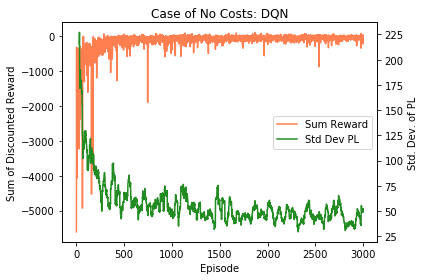
\includegraphics[width=70mm]{../fig/fig01a.png}
  \end{center}
  \subcaption{DQN}
  \label{fig01a}
 \end{minipage}
 \begin{minipage}{0.5\hsize}
  \begin{center}
   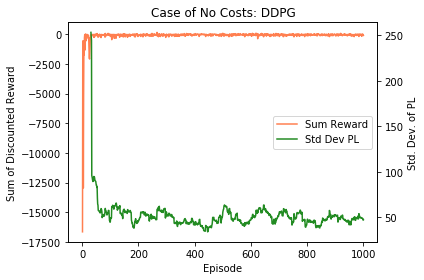
\includegraphics[width=70mm]{../fig/fig01b.png}
  \end{center}
  \subcaption{DDPG}
  \label{fig01b}
 \end{minipage}
 \caption{Learning curves of (a) DQN and (b) DDPG. The standard deviation of PL at each episode is calculated from the last 30 episodes.}
\end{figure}

Figures \ref{fig01a} and \ref{fig01b} are the learning curves of DQN and DDPG, respectively. Each figure shows the histories of the cumulative sum of discounted rewards (orange) and the standard deviation of profit and loss (PL) at the expiry (green), where the standard deviation at each episode is calculated from the last 30 episodes. The sum of rewards should be convergent to zero because the delta hedging is optimal. The standard deviation of PL should be smaller as the learning appropriately proceeds. Figures \ref{fig01a} and \ref{fig01b} suggest that both DQN and DDPG learnings are sufficiently convergent.

\begin{figure}[tb]
	\begin{center}
		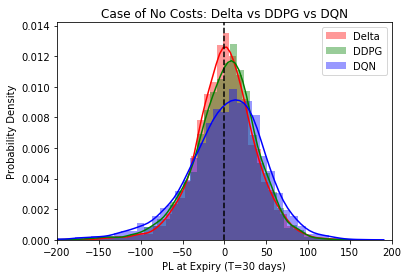
\includegraphics[width=10cm]{../fig/fig02.png}
		\caption{Histograms of PL at the expiry ($t=T$) by the Delta (red), the DDPG (green), and the DQN (blue) agent. The PL is defined by (\ref{PL:expiry}). The PL values are calculated from newly sampled 3000 paths. Each curve represent the kernel density estimation.}
		\label{fig02}
	\end{center}
\end{figure}

Although the optimal policy is the delta hedging \citep{Kolm:Ritter:2019}, the hedge error is not exactly zero due to the discreteness of time \citep{Derman:Miller:2016}. The hedge error of an agent can be measured by the standard deviation of PL at the expiry ($t = T$):
%
\begin{equation}
	{\rm PL}_T := (N_T S_T - N_0 S_0) + (100 C_0 - N_0 S_0) e^{\rho T}
	+ \sum_{t=0}^{T-1} \{B_{t+1} - B_t e^{\rho \delta t}\} e^{\rho (T-t)} - 100 C_T. \label{PL:expiry}
\end{equation}
%
Note that the expectation of PL at the expiry is the first term of the cumulative sum of discounted rewards (\ref{expected:return}). The delta hedging agent (shortly, Delta agent) has the minimum standard deviation of PL because its policy is optimal. Figure \ref{fig02} shows the histograms of PL by the Delta (red), the DDPG (green), and the DQN (blue) agent, which are calculated from newly sampled 3000 paths. The standard deviation of PL by the DDPG agent is smaller than that by the DQN, which means that the DDPG solution is closer to the global optimizer.

The DQN agent has the hidden layers of 16x16 (i.e., two hidden layers, each of which has 16 units). In the DDPG agent, the hidden layers of the actor and the critic are 12x12x12 and 24x24x24, respectively. These facts suggest that the standard deviation of PL by the DQN is larger because its deep network does not have sufficiently large degree of freedom. We perform similar numerical experiments using the DQNs with no hidden layer or the hidden layers of 16x16x16 (three hidden layers) and 16 (one hidden layers). The standard deviation of PL is smallest in the case of the 16x16 hidden layers (i.e., two hidden layers). This suggests that the above result of convergence (Fig. \ref{fig02}) is not sensitive to the DQN architecture.

The DQN agent selects an action from the 101 possible ones, which is the number of shares of stock from 0 to 100. An action of the DQN is determined by $\argmax_{a'} q^\ast(s, a')$. These facts indicate that the action space is too large for the agent to explore sufficiently and it is difficult to estimate $q^\ast$ with high accuracy. In contrast, the DDPG agent determines its action by $a = \mu(s)$. When we use an appropriate function approximation, a DDPG agent does not have to explore the action space in detail. The effective degree of freedom is often smaller than the dimension of action or state space. Such effective degree of freedom is represented by the function parameters, which are tuned by any sample data.

\begin{figure}[htb]
	\begin{center}
		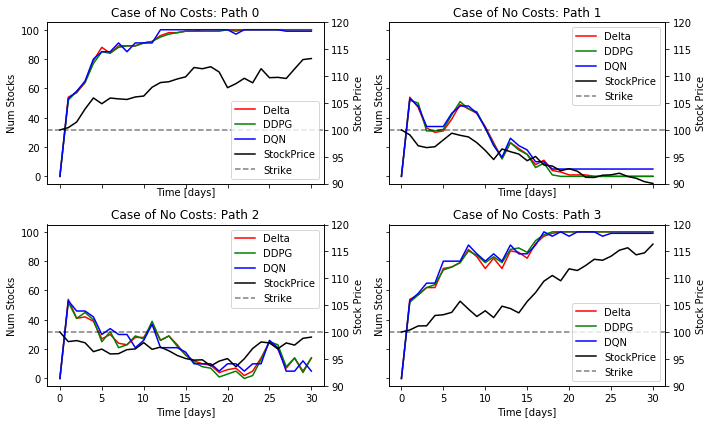
\includegraphics[width=15cm]{../fig/fig03.png}
		\caption{Sample paths. Each figure shows the time series of the number of shares of stock by the Delta (red), the DDPG (green), and the DQN (blue) agent. The time series of stock price is also shown (black). The horizontal dashed lines represent the strike $K$ ($= 100$). In Path 0 and 3, the option is in the money at the expiry ($t=T$), while it is out of the money in Path 1 and 2.}
		\label{fig03}
	\end{center}
\end{figure}

Figure \ref{fig03} shows four sample paths. Each figure shows the time series of the number of shares of stock by the Delta (red), the DDPG (green), and the DQN (blue) agent, together with the time series of stock price (black). The DDPG paths are closer to the Delta paths. This fact can also be confirmed in Fig. \ref{fig04}, which shows the histograms of the difference between the number of shares of stock at various times. The DDPG agent makes the position closer to the delta neutral position at each time. 

\begin{figure}[tb]
	\begin{center}
		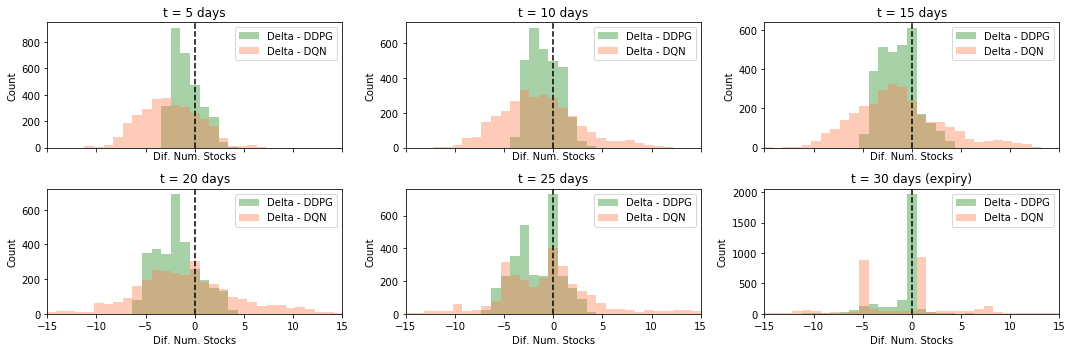
\includegraphics[width=15cm]{../fig/fig04.png}
		\caption{Histograms of the difference between the numbers of shares of stock with no transaction costs. The figures are made from newly sampled 3000 paths.}
		\label{fig04}
	\end{center}
\end{figure}

\subsection{Cases of non-zero transaction costs}

We investigate the cases of non-zero transaction costs: the value of $\alpha$ in (\ref{cost:function}) is $1 \times 10^{-3}$, $4 \times 10^{-3}$, or $8 \times 10^{-3}$. In these cases, the delta hedging is not optimal and we expect that the DDPG or DQN policy is close to be optimal.

\begin{figure}[htb]
	\begin{center}
		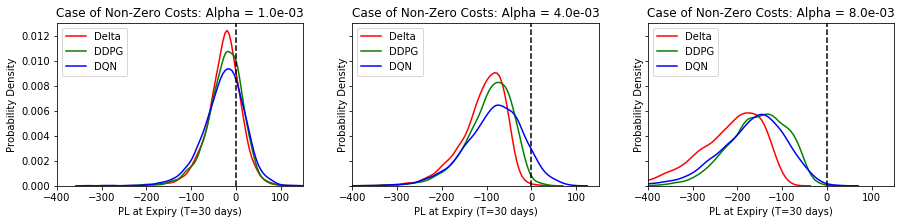
\includegraphics[width=15cm]{../fig/fig05.png}
		\caption{Kernel density estimations of the histograms of PL at the expiry ($t=T$). The estimations are made from newly sampled 3000 paths.}
		\label{fig05}
	\end{center}
\end{figure}

Figure \ref{fig05} shows the kernel density estimations (KDEs) of the histograms of PL at the expiry ($t=T$) by the Delta (red), the DDPG (green), and the DQN (blue) agent. The statistics of PL are displayed in Tables \ref{Table2}, \ref{Table3}, and \ref{Table4}. When $\alpha = 1 \times 10^{-3}$, the Delta agent gives the smallest standard deviation of PL, while the DDPG gives the largest mean of PL. The KDE is overlapped with each other (Fig. \ref{fig05}) and the difference among the agents is not distinct. When $\alpha = 4 \times 10^{-3}$ or $\alpha = 8 \times 10^{-3}$, the delta hedging is obviously not a good policy. Comparing the DDPG and the DQN agent, the DDPG tends to have a smaller standard deviation of PL and a larger 1 percentile PL. The DQN agent has the largest mean of PL when $\alpha = 4 \times 10^{-3}$ likely due to the largest standard deviation, while the mean of PL by the DDPG is largest when $\alpha = 8 \times 10^{-3}$. We further investigate the case of $\alpha = 8 \times 10^{-3}$.

\begin{table}[htb]
	\begin{center}
	\begin{tabular}{| c | c | c | c |} \hline
            Agent & Mean PL & Std. Dev. PL & 1 percentile PL \\ \hline\hline
            Delta & -26.72 & 38.30 & -137.83 \\  \hline
            DDPG & -24.80 & 40.76 & -144.94 \\  \hline
            DQN & -27.18 &  46.44 & -159.23 \\ \hline
        \end{tabular}
        \caption{Statistics of PL at the expiry ($t=T$) with $\alpha = 1 \times 10^{-3}$.}
        \label{Table2}
        \end{center}
\end{table}

\begin{table}[htb]
	\begin{center}
	\begin{tabular}{| c | c | c | c |} \hline
            Agent & Mean PL & Std. Dev. PL & 1 percentile PL \\ \hline\hline
            Delta & -108.67 & 50.60 & -262.38 \\  \hline
            DDPG & -94.00 & 52.49 & -254.46 \\  \hline
            DQN & -83.44 &  64.35 & -254.72 \\ \hline
        \end{tabular}
        \caption{Statistics of PL at the expiry ($t=T$) with $\alpha = 4 \times 10^{-3}$.}
        \label{Table3}
        \end{center}
\end{table}

\begin{table}[htb]
	\begin{center}
	\begin{tabular}{| c | c | c | c |} \hline
            Agent & Mean PL & Std. Dev. PL & 1 percentile PL \\ \hline\hline
            Delta & -217.94 & 74.32 & -437.02 \\  \hline
            DDPG & -154.43 & 64.98 & -326.55 \\  \hline
            DQN & -167.59 &  75.63 & -389.44 \\ \hline
        \end{tabular}
        \caption{Statistics of PL at the expiry ($t=T$) with $\alpha = 8 \times 10^{-3}$.}
        \label{Table4}
        \end{center}
\end{table}

Figure \ref{fig06} shows nine sample paths of the number of shares of stock by the Delta (red), the DDPG (green), and the DQN (blue) agent, together with the time series of stock price (black). Interestingly, the DDPG or DQN agent does not have 100 shares of stock when the option is in the money at $t=T$. The agent reduces the number of shares of stock to cut the transaction costs, which makes a profit over the period. In fact, Table \ref{Table4} shows the 1 percentile PL of the DDPG or DQN agent is much larger than that of the Delta. Figure \ref{fig06} also indicates the following two points:
%
\begin{itemize}
	\item The DDPG agent tends to have a small number of shares of stock in both cases of ITM (in the money) and OTM (out of the money).
	\item The DQN agent changes a number of shares of stock not frequently.
\end{itemize}
%
These two points suggest that the characteristics of the DQN hedging strategy is statistically different from that of the DDPG strategy, though the PL distributions of the DQN and the DDPG are similar when $\alpha = 8 \times 10^{-3}$ (Fig. \ref{fig05}).

\begin{figure}[tb]
	\begin{center}
		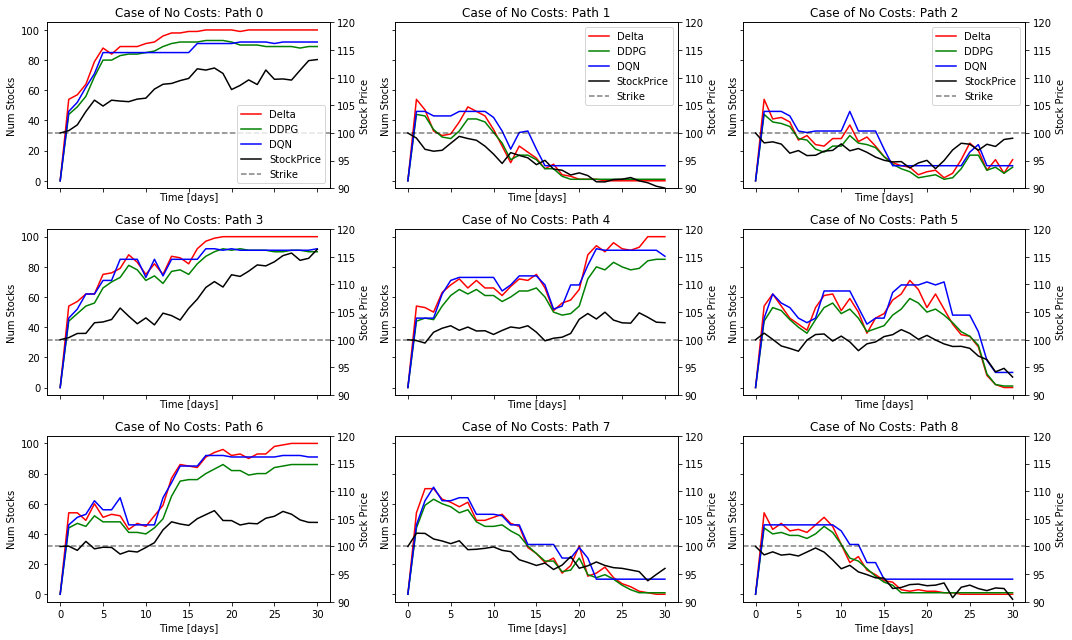
\includegraphics[width=15cm]{../fig/fig06.png}
		\caption{Sample paths with $\alpha = 8 \times 10^{-3}$. Each figure shows the time series of the number of shares of stock by the Delta (red), the DDPG (green), and the DQN (blue) agent. The time series of stock price is also shown (black). The horizontal dashed lines represent the strike $K$ ($= 100$).}
		\label{fig06}
	\end{center}
\end{figure}

Figure \ref{fig07} shows the histograms of the difference between the numbers of shares of stock at various times. The DDPG agent (green) tends to have a smaller number of shares of stock compared to the Delta agent. After $t = 15$ days, the histogram of the DDPG (green) becomes bimodal. The larger peak consists of ITM paths, while the smaller peak (close to zero) consists of OTM paths. As discussed before, the DDPG agent tends not to have 100 stocks even when the option is ITM. The DQN agent (orange) follows the different hedging strategy. Before $t = 20$ days, the DQN tends to have a larger number of shares of stock compared to the Delta agent. The histograms become bimodal after $t = 20$ days: the left peak consists of OTM paths, while the right one consists of ITM paths. When the option is ITM, the DQN agent has a smaller number of stock compared to the Delta agent (like the DDPG agent). In contrast, when the option is OTM, the DQN agent has a larger number of stock compared to the Delta agent. The DQN agent has stocks even when the option is OTM at the expiry. This characteristic can also be confirmed in Fig. \ref{fig06}. This result is likely to reflect that the DQN agent sells or buys stocks not frequently.

\begin{figure}[tb]
	\begin{center}
		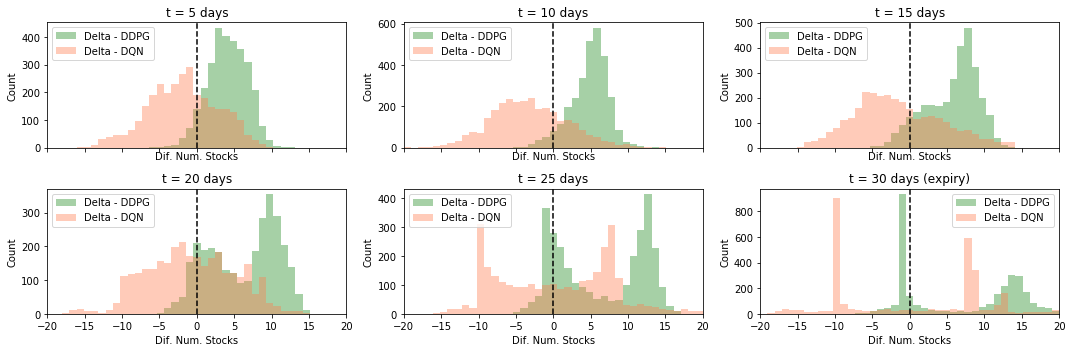
\includegraphics[width=15cm]{../fig/fig07.png}
		\caption{Histograms of the difference between the numbers of shares of stock when $\alpha = 8 \times 10^{-3}$. The histograms are made from newly sampled 3000 paths.}
		\label{fig07}
	\end{center}
\end{figure}

Figure \ref{fig08} shows the histograms of change in the number of shares of stock over a day. We exclude the data within $t = 5$ days because each agent rapidly changes its portfolio from the initial position, which is common to all agents. The Delta agent changes its position most frequently, while the DQN seldom changes its position. Figure \ref{fig08} also suggests that the DQN agent tends to make a large change in the number of shares of stock when rebalancing its portfolio (its histogram has the heaviest tail).

\begin{figure}[htb]
	\begin{center}
		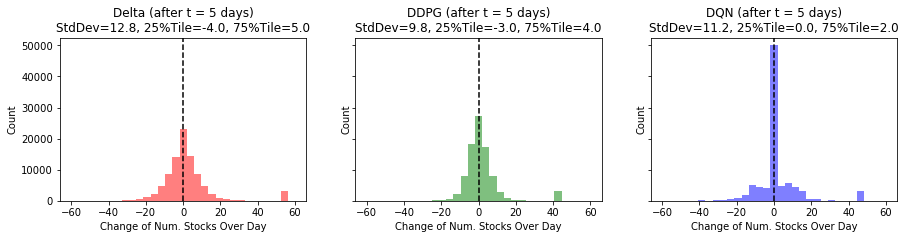
\includegraphics[width=15cm]{../fig/fig08.png}
		\caption{Histograms of change in the number of shares of stock over a day when $\alpha = 8 \times 10^{-3}$ after $t = 5$ days. The histograms are made from newly sampled 3000 paths.}
		\label{fig08}
	\end{center}
\end{figure}

Figure \ref{fig09} shows the scatter plots of the position delta vs the change in the number of shares of stock over a day. The position delta is defined by the number of stock minus the option delta multiplied by 100. For instance, when the position delta is $-50$ [$x = -50$ in Fig. \ref{fig09}], an agent lacks 50 stocks of being delta neutral. The delta agent then buys 50 stocks to make the delta neutral position [$y = 50$ in Fig. \ref{fig09}]. In contrast, the DDPG agent tends to buy or sell smaller number of shares of stock than it would need to make its position delta neutral. The DQN agent does not show such a distinct characteristic and its scatter plot is broad. Although not very clear, sample points by the DQN agent are concentrated around $y=0$, which reflects that the agent buys or sells stocks not frequently.


\begin{figure}[tb]
	\begin{center}
		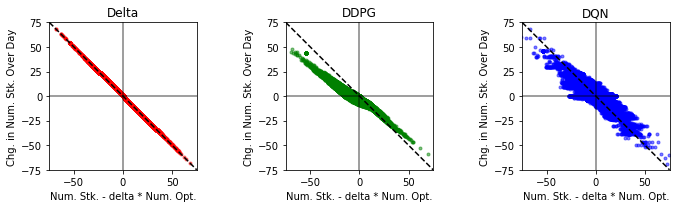
\includegraphics[width=15cm]{../fig/fig09.png}
		\caption{Scatter plots of the position delta vs the change in the number of shares of stock over a day. The position delta is defined by the number of stock minus the option delta multiplied by 100. The plots are made from newly sampled 3000 paths.}
		\label{fig09}
	\end{center}
\end{figure}


\section{Summary}

We have investigated option hedging strategies with the Black-Scholes-Merton (BSM) model with transaction costs, using two reinforcement learning (RL) algorithms: Deep Q Network (DQN) \citep{Watkins:Dayan:1992, Mnih:etal:2013} and Deep Deterministic Policy Gradient (DDPG) \citep{Silver:etal:2014, Lillicrap:etal:2015}. The DQN is simple and applied to a problem with a discrete action space, while the DDPG is complicated and applied to a problem with a continuous action space. An agent hedges 100 call options with strike $K$ and expiry $T$, where the underlying stock price obeys the geometric Brownian motion. We have first considered the case of no transaction costs to examine the convergence of policy. In this case, the optimal policy is delta hedging \citep{Kolm:Ritter:2019}. The DDPG policy is closer to the delta hedging policy than the DQN. We have then examined the cases of non-zero transaction costs. The following characteristics of the DDPG and the DQN agent have been revealed:
%
\begin{itemize}
	\item The DDPG and the DQN agent tend to reduce the number of shares of stock in their positions to cut the transaction costs when the option is in the money (ITM).
	\item The DDPG agent tends to have a smaller number of shares of stock, in the case of not only ITM but also OTM (out of the money).
	\item The DQN agent tends to change a number of shares of stock not frequently.
\end{itemize}

The DQN agent determines a number of shares of stock in its position on the basis of the action-value function $q^\ast(s,a)$. This number (i.e.,  action $a$) must be treated as an integer even if its value is quite large [e.g., $O(10^5)$]. It would be unrealistic to regard the action space as discrete and then the DDPG would be more practical because the DDPG algorithm regards the action space as continuous. Moreover, the DDPG agent has a smaller standard deviation of profit and loss (PL) than the DQN agent in all numerical experiments presented in this report. If we used reinforcement learning techniques in a trading desk, we would construct some weighted averaged policy from various agents including the DQN and the DDPG (i.e., model stacking). The results of this report suggest that a weight of the DDPG is larger than a weigh of the DQN, however, the DQN weight is not zero because the hedging strategy of the DQN is statistically different from that of the DDPG.  Stacking agents with statistically different policies would reduce the variance of rewards and PL. The stacked agent would then determine the amount of extra charge that is added to the BSM fair price from the distribution of PL at the expiry.

\clearpage
\bibliographystyle{unsrt}
\bibliography{references}

\end{document}










